\documentclass[12pt]{ctexart}
    %%% Document Settings %%%%
%\usepackage[utf8]{inputenc}

\usepackage[
    twoside,
    top=1in,
    bottom=0.75in,
    inner=0.5in,
    outer=0.5in,
]{geometry}
\pagestyle{myheadings}
\usepackage{minted}
\usepackage[dvipsnames,svgnames]{xcolor}

%%%% Additional Commands to Load %%%%
\usepackage{tcolorbox}
\tcbuselibrary{skins}
\tcbuselibrary{minted}
\usemintedstyle{lovelace}
%\usepackage{minted}
\usepackage{color}
\usepackage{tikz}
\usetikzlibrary{calc}
\usepackage{tabularx,colortbl}
\usepackage{amsfonts,amsmath,amssymb}
\usepackage{titling}
\usepackage{mathrsfs}
\usepackage{calc}
\usepackage{subcaption}

\usepackage{listings}
%\usepackage{newtxtext}
\usepackage[strict]{changepage} 
\usepackage{framed}
\definecolor{formalshade}{rgb}{0.95,0.95,1}
\usepackage{float}

%%%% Commands to Define Homework Boxes %%%%
%%%% Box Definition %%%%
\newtcolorbox{prob}[1]{
% Set box style
    sidebyside,
    sidebyside align=top,
% Dimensions and layout
    width=\textwidth,
    toptitle=2.5pt,
    bottomtitle=2.5pt,
    righthand width=0.20\textwidth,
% Coloring
    colbacktitle=gray!30,
    coltitle=black,
    colback=white,
    colframe=black,
% Title formatting
    title={
        #1 \hfill Grade:\phantom{WWWW}
    },
    fonttitle=\large\bfseries
}

%%%% Environment Definition %%%%
\newenvironment{problem}[1]{
    \begin{prob}{#1}
}
{
    \tcblower
    \centering
    \textit{\scriptsize\bfseries Faculty Comments}
    \vspace{\baselineskip}
    \end{prob}
}

\newenvironment{formal}{%
\def\FrameCommand{%
\hspace{1pt}%
{\color{DarkBlue}\vrule width 2pt}%
{\color{formalshade}\vrule width 4pt}%
\colorbox{formalshade}%
}%
\MakeFramed{\advance\hsize-\width\FrameRestore}%
\noindent\hspace{-4.55pt}% disable indenting first paragraph
\begin{adjustwidth}{}{7pt}%
\vspace{2pt}\vspace{2pt}%
}
{%
\vspace{2pt}\end{adjustwidth}\endMakeFramed%
}

    \title{特殊方程作业10}
    \author{地物2201班\ 杨曜堃}
    \date{\today}
%%% document
\begin{document}

% Format Running Header
    \markboth{\theauthor}{\thetitle}
    \maketitle
    \begin{description}
        \item[问题1] 采用拉普拉斯变换法求解下列热传导方程的定解问题$$
        \begin{cases}
            \dfrac{\partial u}{\partial t}=a^2\dfrac{\partial^2u}{\partial x^2},&\ 0<x<\infty,\ t>0\\
            u|_{t=0}=T_0\\
            u|_{x=0}=0\\
            u(x,t)|_{x=+\infty}\text{有界}
        \end{cases}$$
    \end{description}
    \begin{problem}{问题\#1}
        对$u(x,t)$做关于$t$的拉普拉斯变换,定义
        $$
        U(x,s)\triangleq \mathscr{L}\left\{u(x,t)\right\}=\int^{+\infty}_{0}u(x,t)e^{-st}\text{d}s
        $$
        根据拉普拉斯变换的微分性质
        $$
        \mathscr{L}\left\{\dfrac{\partial u}{\partial t}\right\}=s\mathscr{L}\left\{u(x,t)\right\}-u(x,0)=sU(x,s)-T_0
        $$
        另一边
        $$
        \mathscr{L}\left\{\dfrac{\partial^2u}{\partial x^2}\right\}=\dfrac{\text{d}U(x,s)}{\text{d}x^2}
        $$
        代入偏微分方程得到非齐次线性偏微分方程
        $$
        \dfrac{\text{d}^2U(x,s)}{\text{d}x^2}-\dfrac{s}{a^2}U(x,s)=-\dfrac{T_0}{a^2}
        $$
        对应齐次方程为
        $$
        \dfrac{\text{d}^2U(x,s)}{\text{d}x^2}-\dfrac{s}{a^2}U(x,s)=0
        $$
    \end{problem}
    \begin{problem}{问题\#1}
        解之,得到齐次方程的通解
        $$
        \widetilde{U}(x,s)=C_1e^{-\frac{\sqrt{s}}{a}x}+C_2e^{\frac{\sqrt{s}}{a}x}
        $$
        我们确信$u(x,t)$在$t>0$不含冲激函数以及高阶奇异函数,因此可以利用拉普拉斯变换的初值定理,即
        $$
        \lim_{s\to \infty}sU(x,s)=u(x,0^+)=T_0
        $$
        说明
        $$
        \lim_{s\to \infty}U(x,s)=0
        $$
        这要求$C_2=0$,即$\widetilde{U}(x,s)=C_1e^{-\frac{\sqrt{s}}{a}x}$。注意到非齐次方程的非齐次项为常数,因此很自然想到非齐次方程的特解为一个常数
        $$
        U^\ast (x,s)=-\dfrac{T_0}{s}
        $$
        根据条件$u(x,t)=0$,得知$U(x,s)=0$,因此可得$C_1=\dfrac{T_0}{s}$。非齐次方程的通解为为
        $$
        U(x,s)=\dfrac{T_0}{s}e^{-\frac{\sqrt{s}}{a}x}-\dfrac{T_0}{s}
        $$
        对该解做拉普拉斯逆变换,根据线性性质
        $$
        \mathscr{L}^{-1}\left\{U(x,s)\right\}=T_0\mathscr{L}^{-1}\left\{\dfrac{1}{s}e^{-\frac{\sqrt{s}}{a}x}\right\}-T_0\mathscr{L}^{-1}\left\{\dfrac{1}{s}\right\}
        $$
        对于第二项可以轻松得到$\mathscr{L}^{-1}\left\{\dfrac{1}{s}\right\}=1$,因此重点关注第一项。根据黎曼-梅林反演公式
        \begin{formal}
            $$
            \mathscr{L}^{-1}\left\{\dfrac{1}{s}e^{-\frac{\sqrt{s}}{a}x}\right\}=\dfrac{1}{2\pi j}\int^{\sigma+j\infty}_{\sigma-j\infty}\dfrac{1}{s}e^{-\frac{\sqrt{s}}{a}x}e^{st}\mathrm{d}s
            $$
        \end{formal}
        为了求解该积分,需要构造函数
        $$
        f(z)=\dfrac{1}{s}e^{-\frac{\sqrt{z}}{a}x}e^{zt}
        $$
        取$\sigma>0$,规定$z$的辐角取值范围在$(-\pi,\pi]$,取围道如图所示
    \end{problem}
    \begin{problem}{问题\#1}
        \begin{center}
            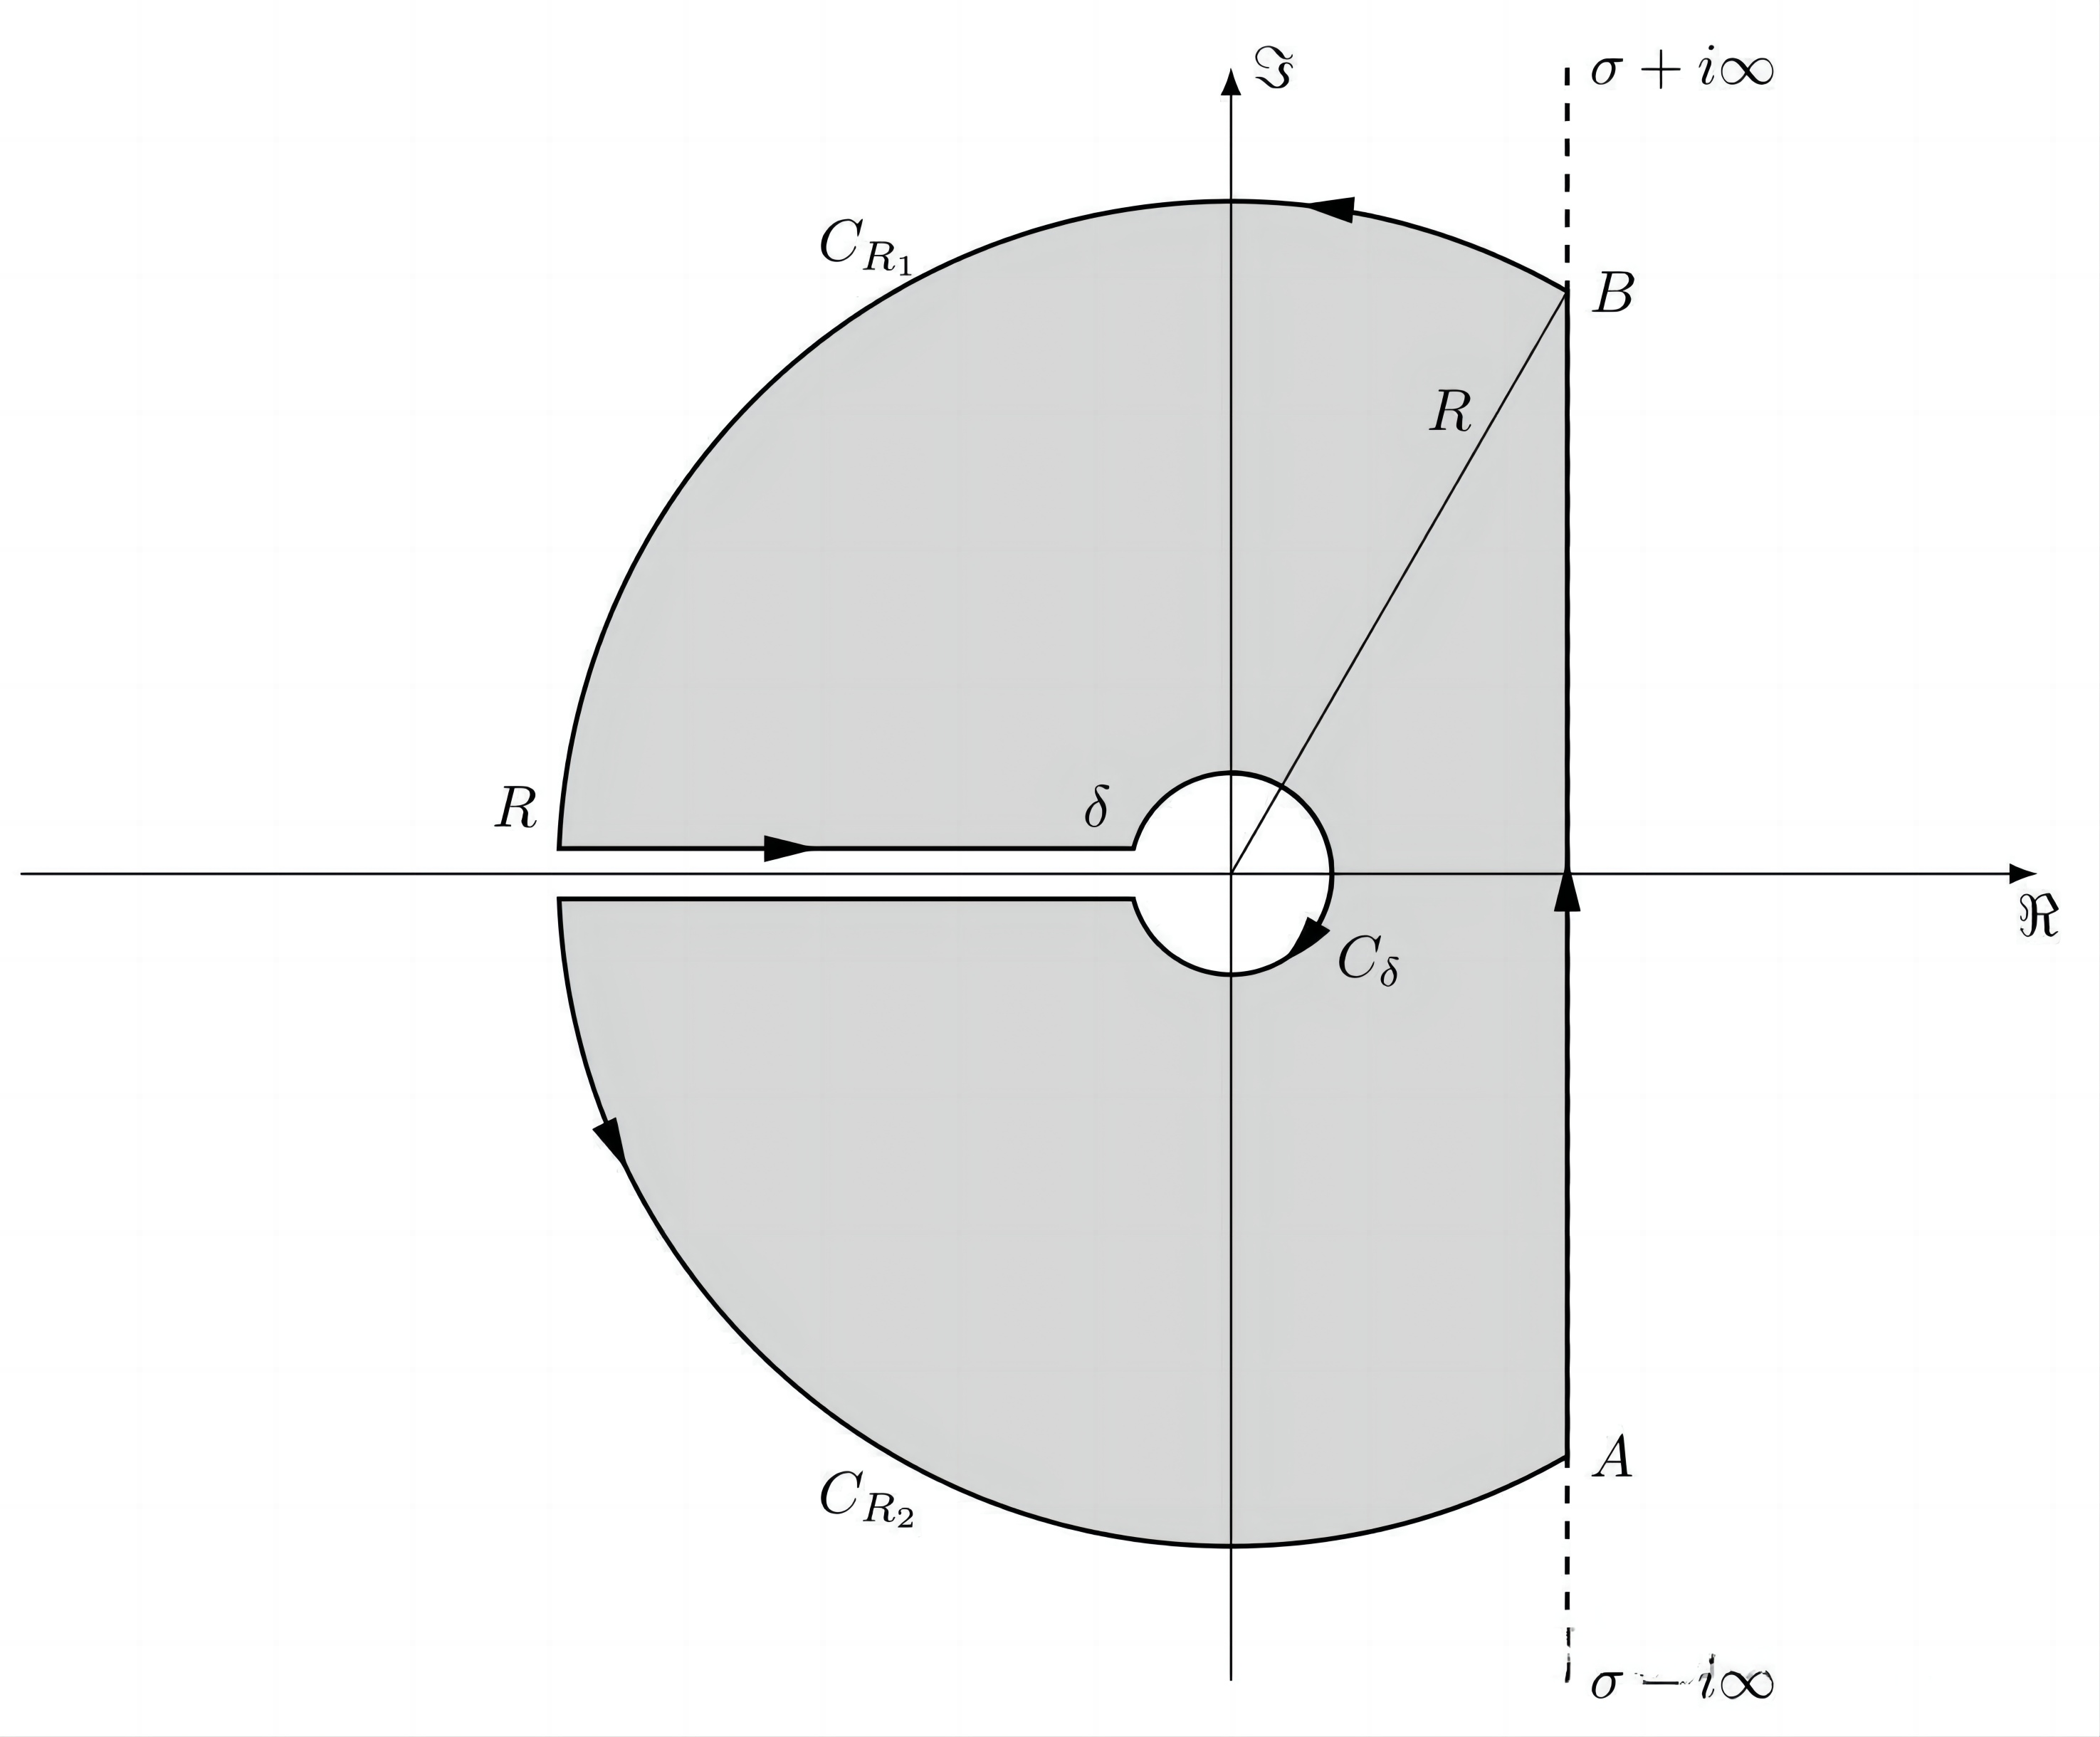
\includegraphics[width=8cm]{fig1.png}
        \end{center}
        $z=0$是$f(z)$的一个支点,因此围道需要沿实轴割开。$f(z)$在围道内是可解析的,根据留数定理
        $$
        \left(\int^{B}_{A}+\int_{C_{R_{1}}}+\int^{\delta}_{R}+\int_{C_{\delta}}+\int^{R}_{\delta}+\int_{C_{R_{2}}}\right)f(z)\mathrm{d}z=0
        $$
        观察被积函数$f(z)$中指数上的实部
        $$
        \mathrm{Re} \left\{-\sqrt{Re^{j\theta}+Re^{j\theta t}}\right\}=Rt\cos\theta-\sqrt{R}\cos\dfrac{\theta}{2}<0
        $$
        因此针对$C_{R_1}$上的积分
        $$
        \lim_{R\to\infty}\int_{C_{R_{1}}}f(z)\mathrm{d}z=0
        $$
        同理针对$C_{R_2}$上的积分
        $$
        \lim_{R\to\infty}\int_{C_{R_{2}}}f(z)\mathrm{d}z=0
        $$
        对于$C_\delta$上的积分,也可以判断出
        $$
        \lim_{\delta\to0}\int_{C_{\delta}}f(z)\mathrm{d}z=0
        $$
        此时还剩下两个积分,可以计算
        $$
        \lim_{R\to\infty,\ \delta\to0
            }
                \int^{\delta}_{R}f(ye^{\pi j})\mathrm{d}y=
                -\int^{\infty}_{0}\dfrac{e^{-j\frac{\sqrt{y}}{a}x}}{y}e^{-yt}\mathrm{d}y
        $$
    \end{problem}
    \begin{problem}{问题\#1}
        $$
        \lim_{R\to\infty,\ \delta\to0
        }
            \int^{\delta}_{R}f(ye^{\pi j})\mathrm{d}y=
            -\int^{\infty}_{0}\dfrac{e^{-j\frac{\sqrt{y}}{a}x}}{y}e^{-yt}\mathrm{d}y
        $$
        这里的$y$只是作为积分变量,不具备实际物理意义。两式相加即可得到
        $$
        \lim_{R\to\infty,\ \delta\to0
        }
        \left(
            \int^{\delta}_{R}f(z)\mathrm{d}z+\int^{R}_{\delta}f(z)\mathrm{d}z
        \right)=2j\int^{\infty}_{0}\dfrac{\sin\frac{\sqrt{y}}{a}x}{y}e^{-yt}\mathrm{d}y
        $$
        从而便可计算出黎曼-梅林反演公式的结果
        $$
        \dfrac{1}{2\pi j}\int^{\sigma+j\infty}_{\sigma-j\infty}\dfrac{1}{s}e^{-\frac{\sqrt{s}}{a}x}e^{st}\mathrm{d}s=-\dfrac{1}{\pi}
        {\color{red}
        \int^{\infty}_{0}\dfrac{\sin\frac{\sqrt{y}}{a}x}{y}e^{-yt}\mathrm{d}y
        }
        $$
        红色部分积分求解非常困难,其中一种思路是利用帕塞瓦尔定理(傅里叶变换是酉变换),先令$y=u^2$进行换元
        $$
        \int^{\infty}_{0}\dfrac{\sin\frac{\sqrt{y}}{a}x}{y}e^{-yt}\mathrm{d}y=
        \int^{\infty}_{-\infty}\dfrac{\sin\frac{xu}{a}}{u}e^{-u^2t}\mathrm{d}u
        $$
        然后计算$\frac{1}{u}$的傅里叶变换和$\sin\frac{xu}{a}e^{-u^2t}$的傅里叶逆变换。这一方法比较麻烦,需要再次利用留数定理计算围道积分以及高斯积分公式,所以这里只给出有用的计算结果
        $$
        \mathscr{L}^{-1}\left\{\dfrac{1}{s}e^{-\frac{\sqrt{s}}{a}x}\right\}=\text{erfc}\left(\dfrac{x}{2a\sqrt{t}}\right)
        $$
        也可以通过查阅积分表得知
        \begin{formal}
            $$
            \begin{aligned}
                \int^{\infty}_{0}\dfrac{e^{-{p+x}y}}{\pi(p+x)}\sin(a\sqrt{x})\mathrm{d}x&=
                -\sinh(a\sqrt{p})+\dfrac{e^{-a\sqrt{p}}}{2}\text{erf}\left(\dfrac{a}{2\sqrt{y}}-\sqrt{py}\right)\\
                &+\dfrac{e^{a\sqrt{p}}}{2}\text{erf}\left(\dfrac{a}{2\sqrt{y}}+\sqrt{py}\right)
            \end{aligned}
            $$
        \end{formal}
        两种方法效果是一样的,最终都可以得到结果
        $$
        u(x,t)=T_0\ \text{erfc}\left(\dfrac{x}{2a\sqrt{t}}\right)+T_0
        $$

    \end{problem}
    % \begin{lstlisting}[language = Matlab,title={test4\_script.m},  numbers=left, 
    %     numberstyle=\tiny,keywordstyle=\color{blue!70},
    %     commentstyle=\color{red!50!green!50!blue!50},frame=shadowbox,
    %     rulesepcolor=\color{red!20!green!20!blue!20},basicstyle=\ttfamily]
    % \end{lstlisting}
    % \begin{figure}[htbp]
    %     \small
    %     \centering
    %     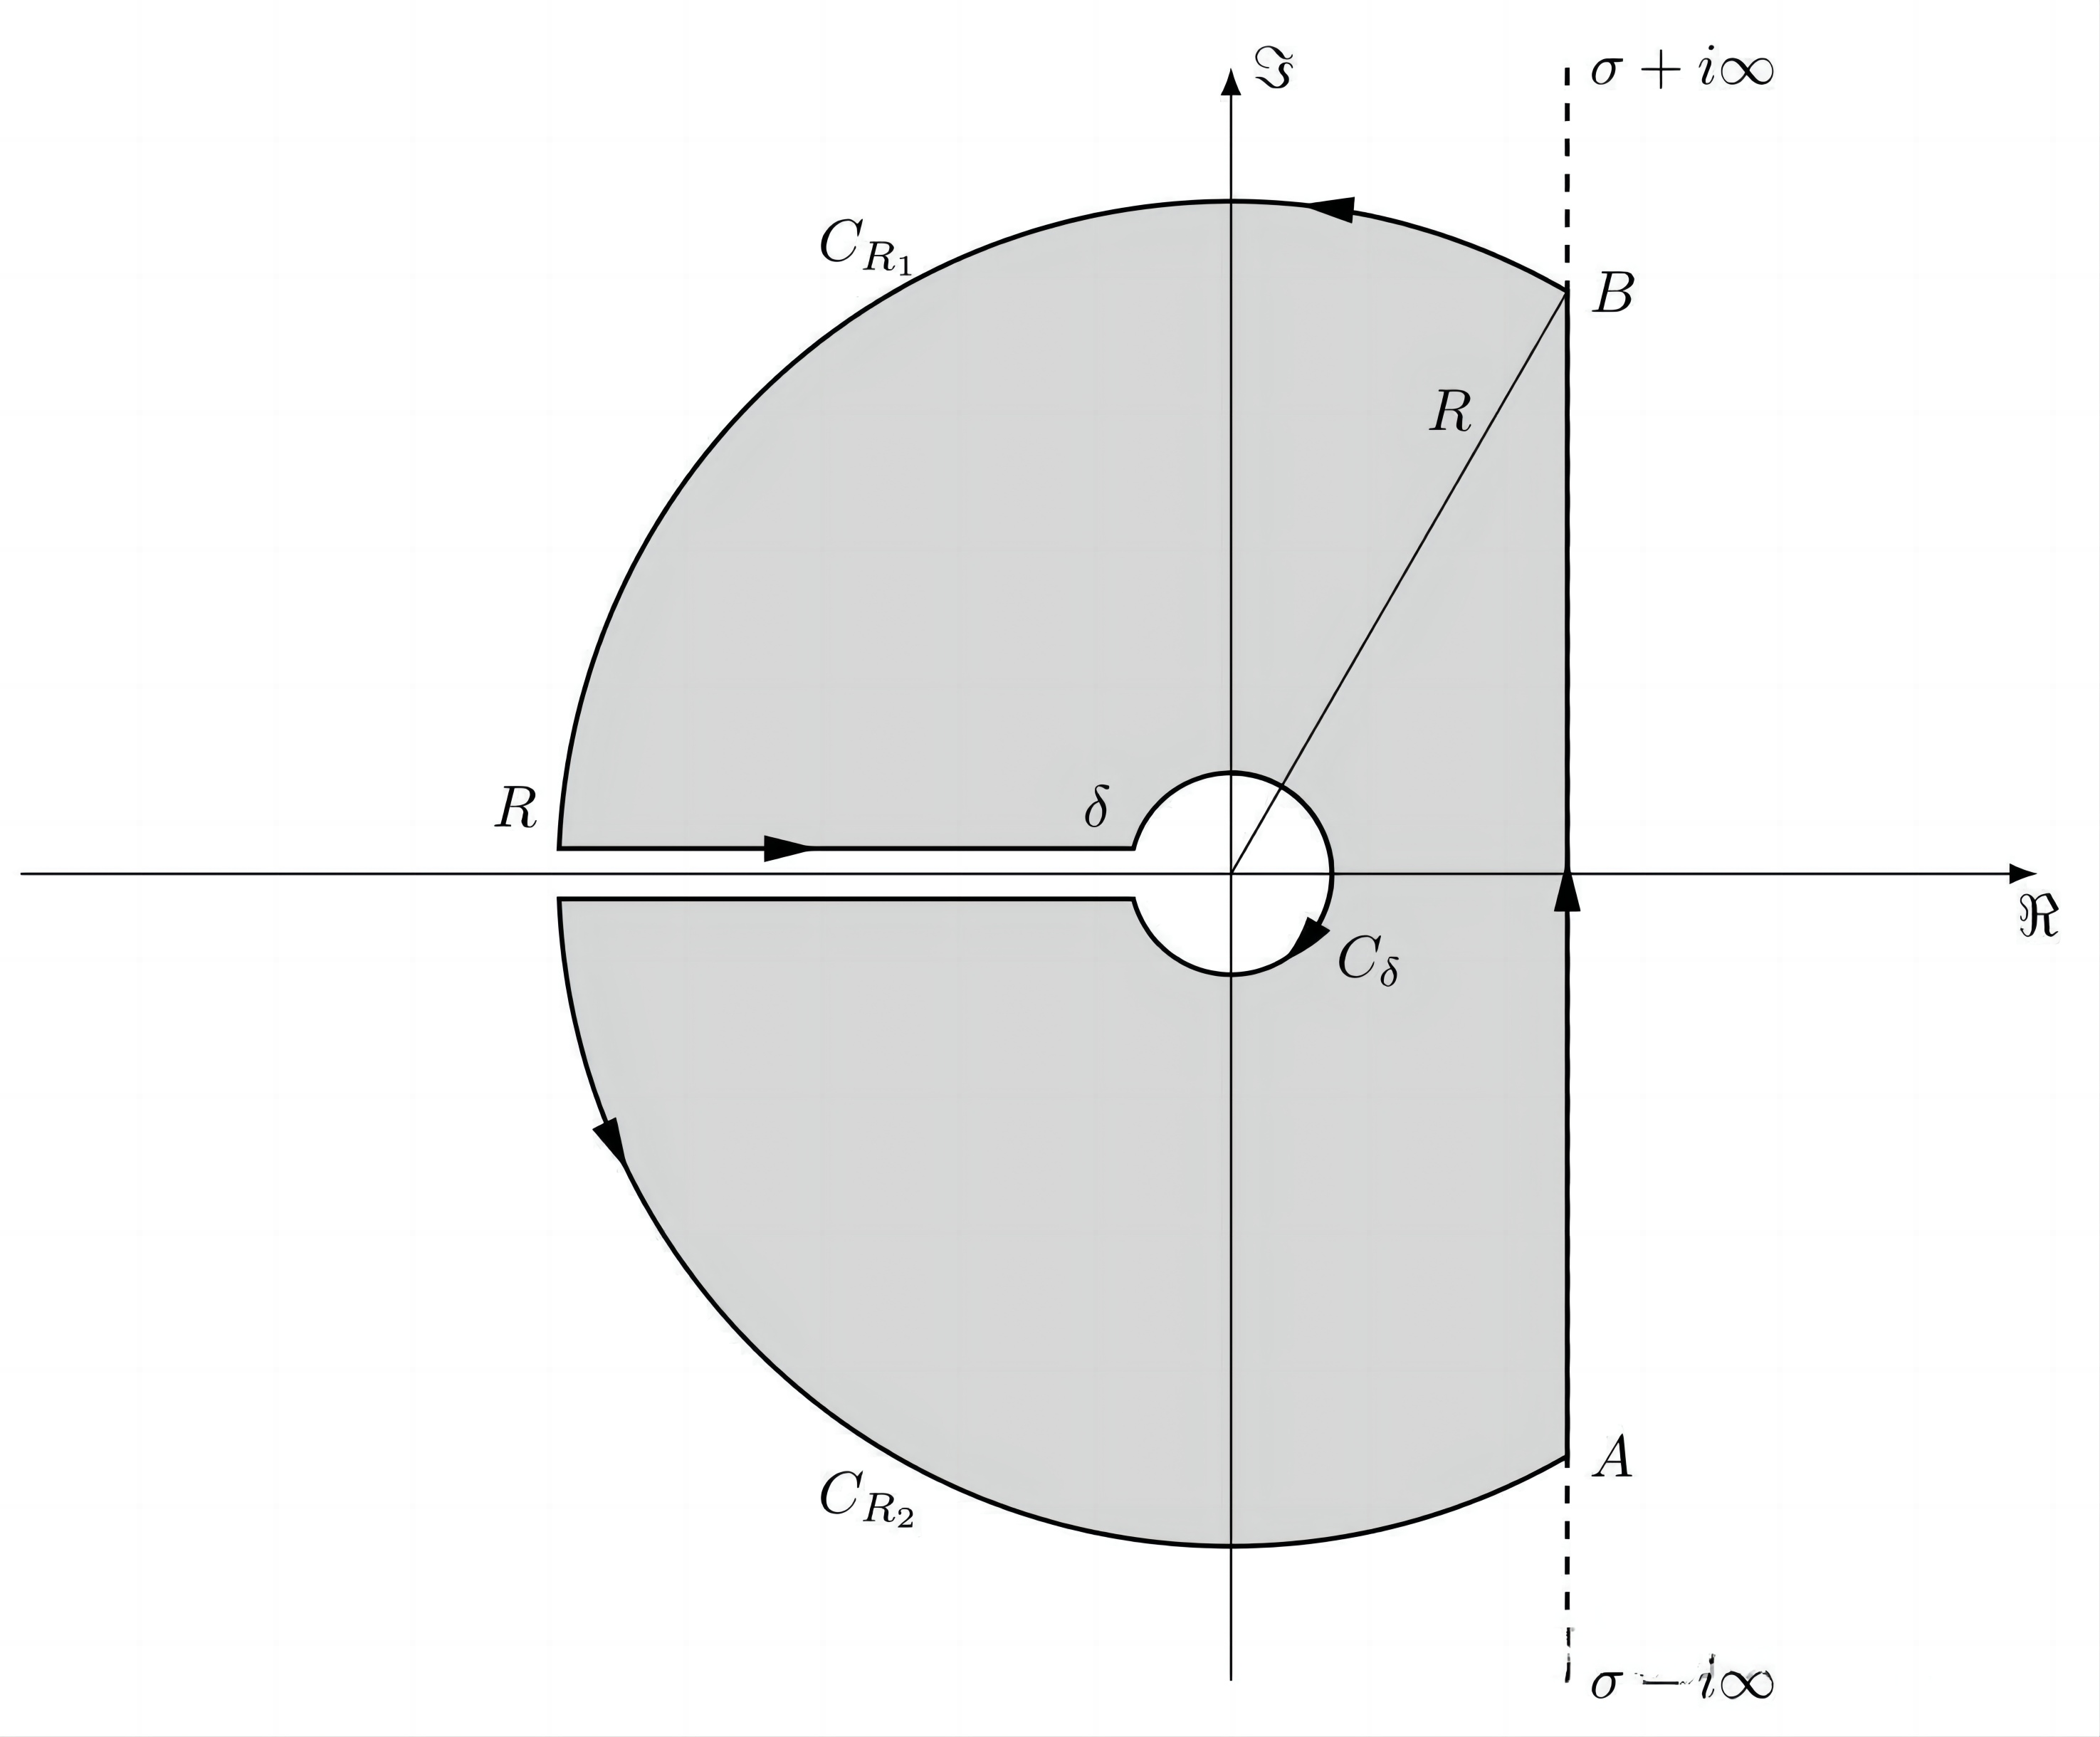
\includegraphics[width=16cm]{fig1.png}
    %     \caption{第一题结果图} \label{Fig:aa}
    % \end{figure}
\end{document}